\documentclass[tikz,border=8pt]{standalone}
\usepackage{pgfplots}
\pgfplotsset{compat=1.18}
\begin{document}
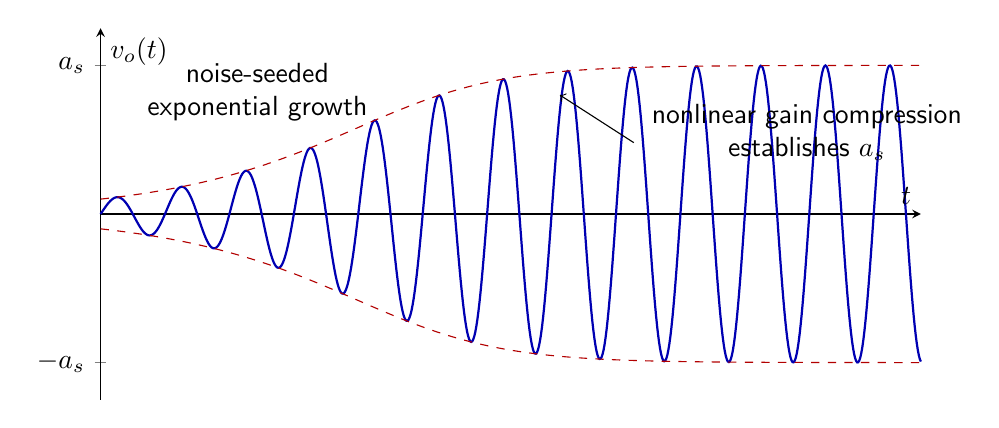
\begin{tikzpicture}[font=\sffamily]
\begin{axis}[width=12cm,height=6.3cm,axis lines=middle,xlabel={$t$},ylabel={$v_o(t)$},xmin=0,xmax=10,ymin=-1.25,ymax=1.25,xtick=\empty,ytick={-1,0,1},yticklabels={$-a_s$,0,$a_s$},samples=800,domain=0:10,clip=false]
\addplot[blue!70!black,thick] {sqrt(1/(1+99*exp(-1.25*x)))*sin(deg(8*x))};
\addplot[red!70!black,dashed] {sqrt(1/(1+99*exp(-1.25*x)))};
\addplot[red!70!black,dashed] {-sqrt(1/(1+99*exp(-1.25*x)))};
\node[align=center,anchor=west] at (axis cs:6.6,.55) {nonlinear gain compression\\establishes $a_s$};
\draw[->] (axis cs:6.5,.48) -- (axis cs:5.6,.8);
\node[align=center,anchor=west] at (axis cs:.45,.82) {noise-seeded\\exponential growth};
\end{axis}
\end{tikzpicture}
\end{document}
